\chapter{Expectation, Information, and Conditioning}\label{ch:expectation-conditioning}
\section{Expectation}
Let $X$ be a random variable defined on a probability space $(\Omega, \F, \Prob)$. We would like to compute an ``average value'' of $X$, taking the probabilities into account when averaging. If $\Omega$ is finite, we simply define this average value by
\[
\E[X] = \sum_{\omega \in \Omega} X(\omega)\,\Prob(\{\omega\}).
\]
If $\Omega$ is \textbf{countably infinite}, its elements can be listed in a sequence $\omega_1, \omega_2, \omega_3, \ldots$, and (provided the series converges absolutely) we can define $\E[X]$ as an infinite sum:
\[
\E[X] = \sum_{k=1}^{\infty} X(\omega_k)\,\Prob(\{\omega_k\}).
\]

However, if $\Omega$ is \textbf{uncountably infinite}, we cannot list its elements in a sequence, and uncountable sums cannot be defined in this way.

\subsection*{Riemann Integral Revisited}
If $f(x)$ is a continuous function defined for all $x$ in the closed interval $[a, b]$, we define the Riemann integral $\int_a^b f(x)\dd x$ as follows. First partition $[a, b]$ into subintervals $[x_0, x_1], [x_1, x_2], \ldots, [x_{n-1}, x_n]$, where $a = x_0 < x_1 < \cdots < x_n = b$. We denote by $\Pi = \{x_0, x_1, \ldots, x_n\}$ the set of partition points and by
\[
\|\Pi\| = \max_{1 \leq k \leq n} (x_k - x_{k-1})
\]
the \textbf{mesh} (length of the longest subinterval) of the partition. For each subinterval $[x_{k-1}, x_k]$, we set $M_k = \max_{x_{k-1} \leq x \leq x_k} f(x)$ and $m_k = \min_{x_{k-1} \leq x \leq x_k} f(x)$. The upper Riemann sum is
\[
\operatorname{Riemann\ Sum}_{\Pi}^{+}(f) = \sum_{k=1}^n M_k (x_k - x_{k-1}),
\]
and the lower Riemann sum is
\[
\operatorname{Riemann\ Sum}_{\Pi}^{-}(f) = \sum_{k=1}^n m_k (x_k - x_{k-1}).
\]
\begin{definition}\label{def:riemann-integral}
    As $\|\Pi\|$ converges to zero, the upper Riemann sum and the lower Riemann sum converge to the same limit, which we denote by $\int_a^b f(x)\dd x$. This common limit is the \textbf{Riemann integral}.
\end{definition}
\begin{figure}[!htpb]
    \centering
    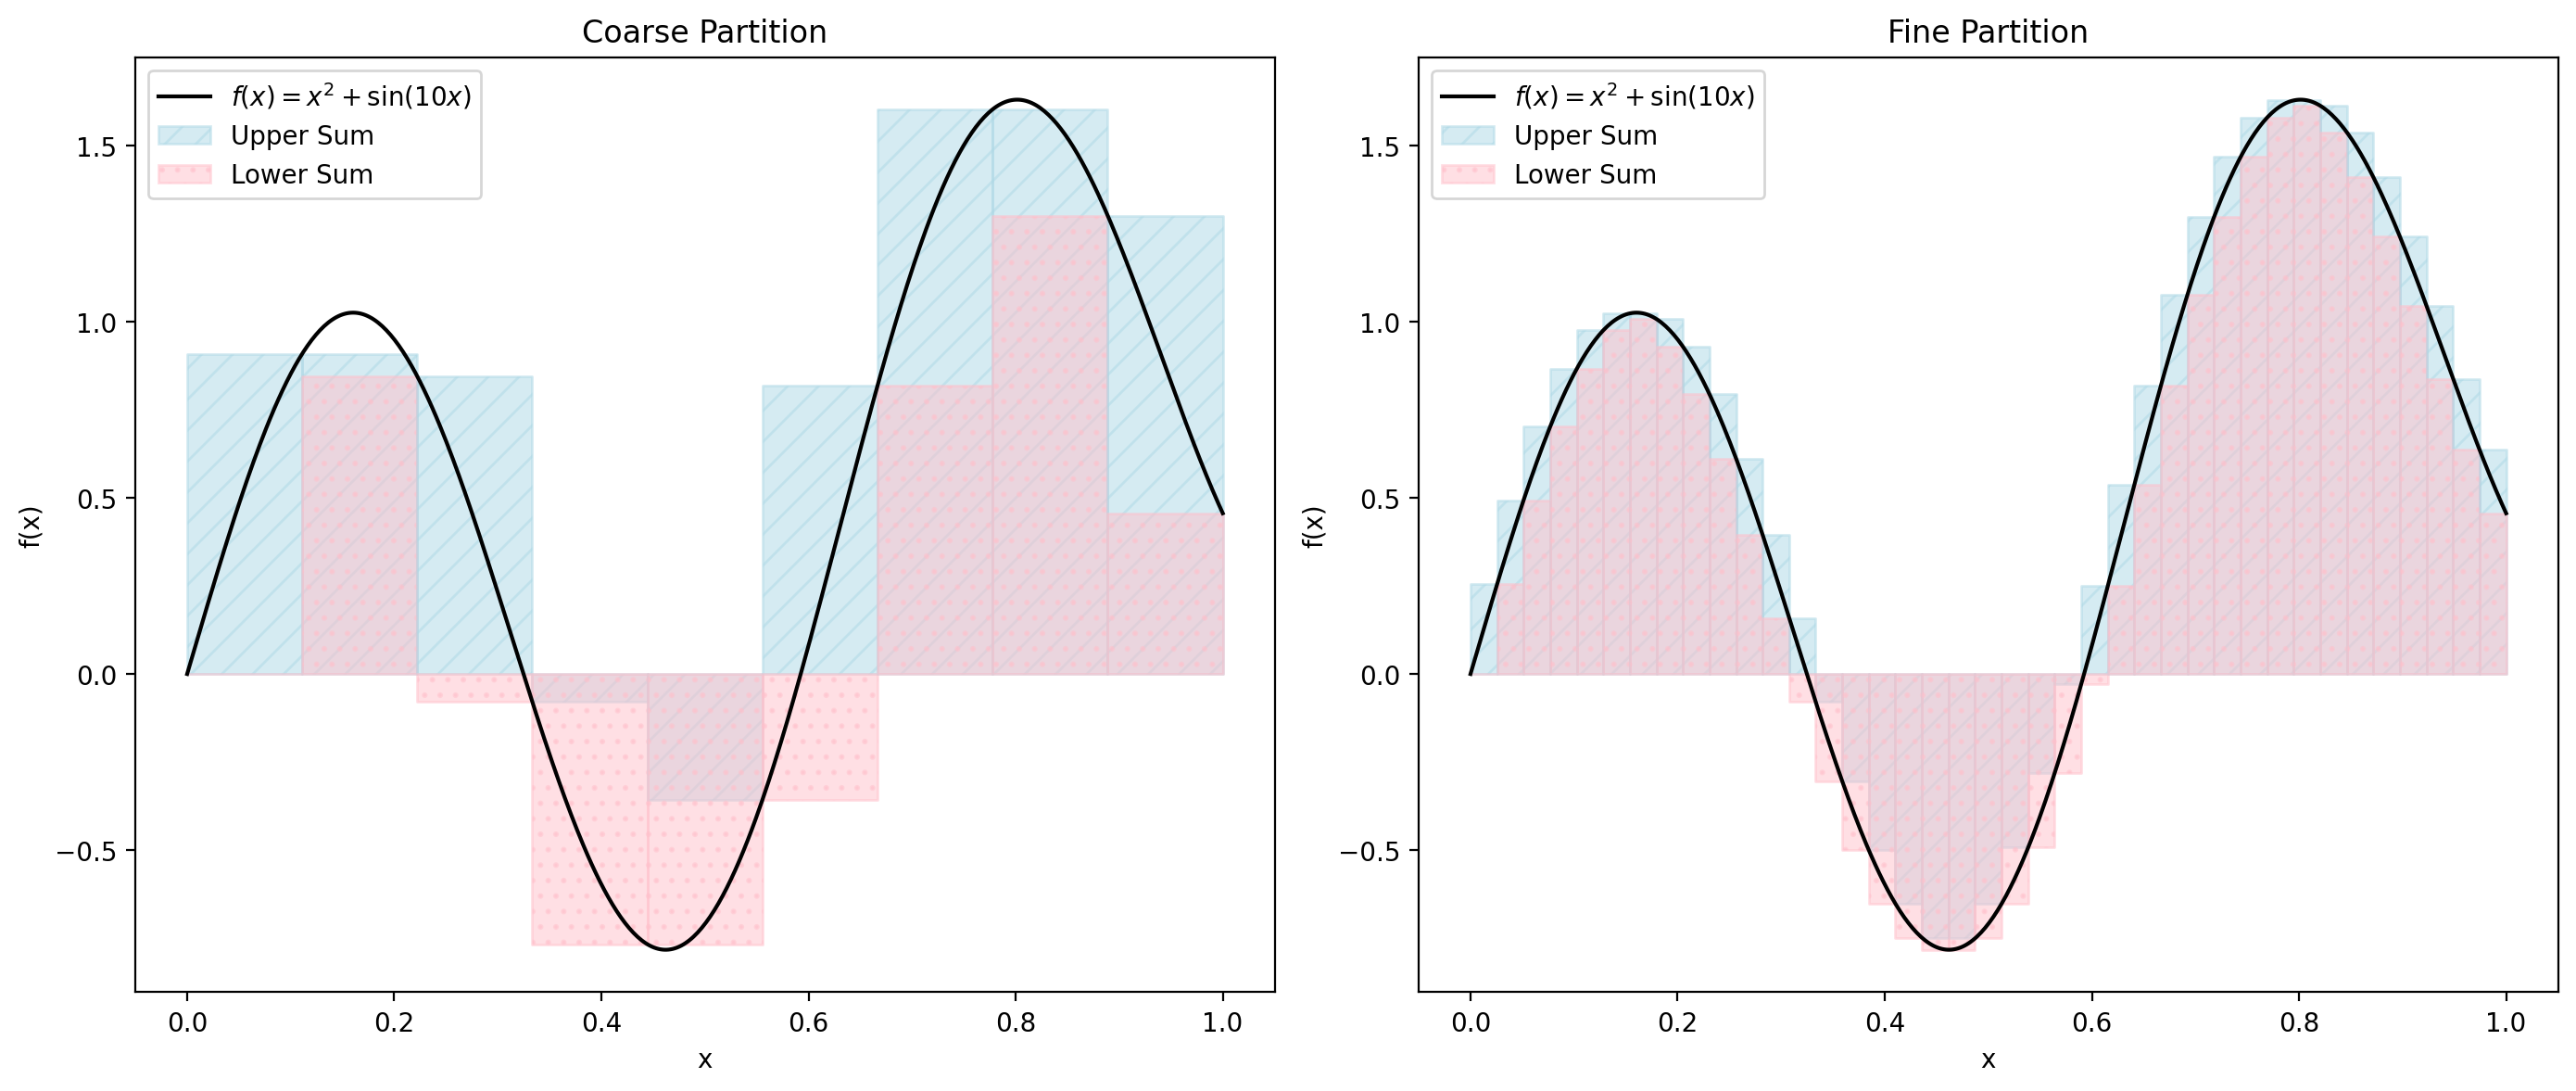
\includegraphics[width=0.8\textwidth]{Figure/RM_integral.png}
    \caption{Riemann Integral}\label{fig:riemann-integral}
\end{figure}

\subsection*{Lebesgue Integral}
Recall that a random variable is a measurable function $X : \Omega \to \R$, where $\Omega$ is the sample space. The difficulty with imitating the Riemann procedure to define expectation is that $X$, unlike the function $f$ above, is defined on an abstract space $\Omega$ that is often not a subset of $\R$. In Figure~\ref{fig:lebesgue-integral}, the ``$x$-axis'' is not the real line but an abstract space $\Omega$, so there is no natural way to partition $\Omega$ as we partitioned $[a, b]$ in Figure~\ref{fig:riemann-integral}. Therefore, we partition the $y$-axis instead.

Assume for the moment that $0 \leq X(\omega) < \infty$ for every $\omega \in \Omega$, and let $\Pi = \{y_0, y_1, y_2, \ldots\}$ be a partition of $[0, \infty)$ such that $0 = y_0 < y_1 < y_2 < \cdots$ with $\lim_{k \to \infty} y_k = \infty$. For each subinterval $[y_k, y_{k+1})$ ($k = 0, 1, 2, \ldots$), we set
\[
A_k = \{\omega \in \Omega : y_k \leq X(\omega) < y_{k+1}\}.
\]

In the Riemann integral, the measure of a subinterval along the $x$-axis is its length, and the height along the $y$-axis is the value of the function. Here, the measure of the corresponding event along the horizontal axis is its probability $\Prob(A_k)$. Therefore, we define the lower Lebesgue sum to be
\[
\operatorname{Lebesgue\ Sum}_{\Pi}^{-}(X) = \sum_{k=0}^{\infty} y_k\,\Prob(A_k).
\]
\begin{figure}[!htpb]
    \centering
    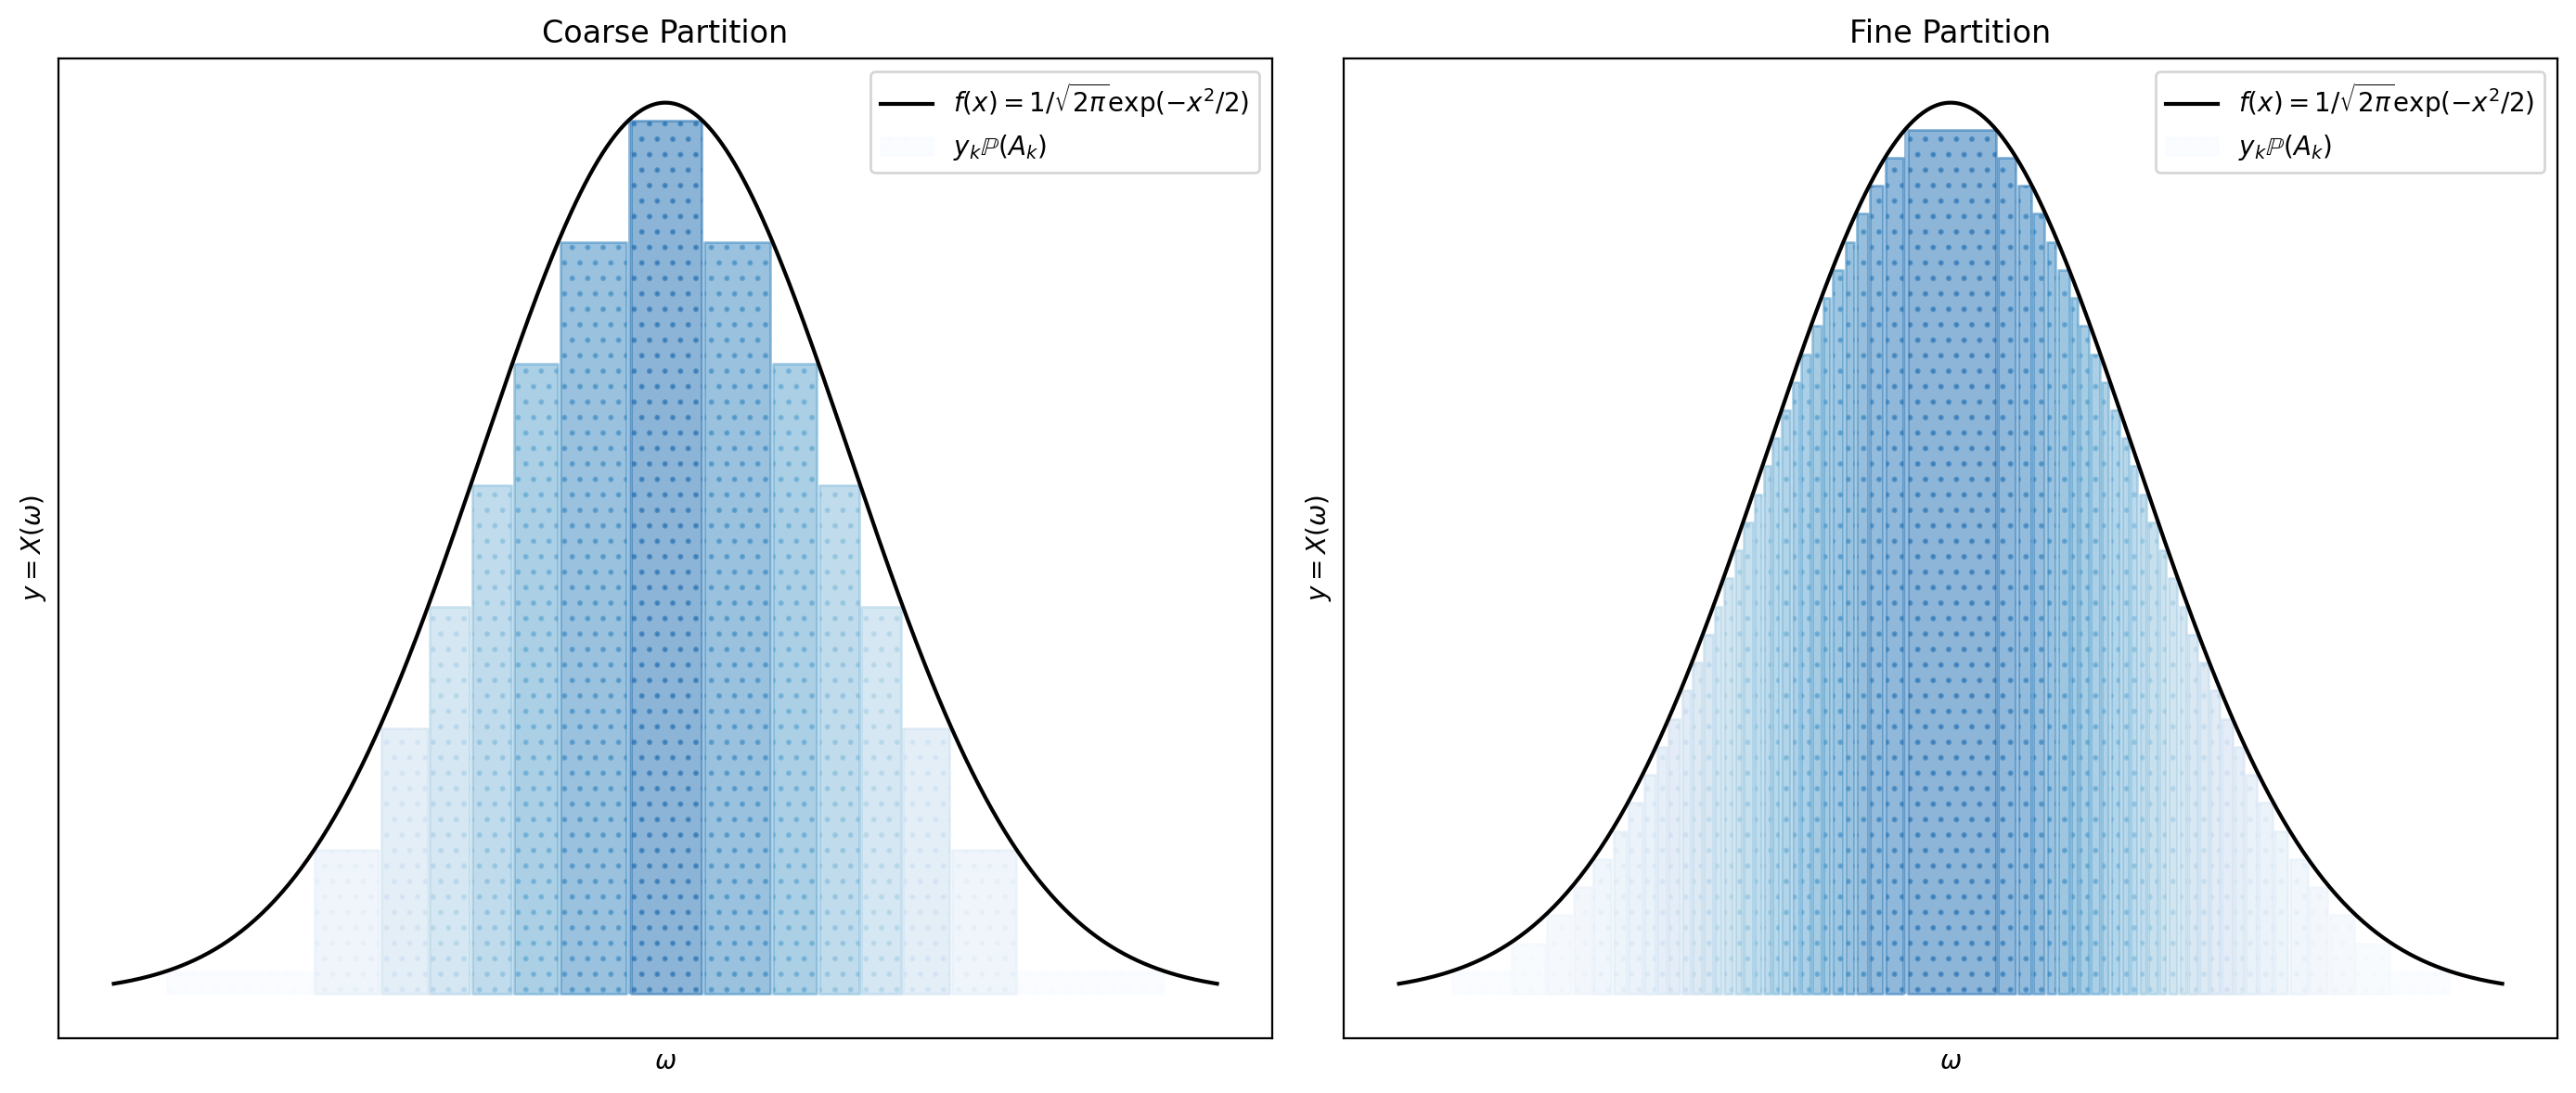
\includegraphics[width=0.8\textwidth]{Figure/Lebesgue.png}
    \caption{Lebesgue Integral}\label{fig:lebesgue-integral}
\end{figure}

As $\|\Pi\| = \sup_{k \geq 0} (y_{k+1} - y_k)$ approaches zero (with $y_k \to \infty$), this lower sum converges to a limit in $[0, \infty]$, which we define to be the \textbf{Lebesgue integral} $\int_{\Omega} X(\omega)\dd\Prob(\omega)$, or simply $\int_{\Omega} X\dd\Prob$. The Lebesgue integral may equal $+\infty$, because we have not placed any bound on how large the values of $X$ can be.

We assumed above that $0 \leq X(\omega) < \infty$ for every $\omega \in \Omega$. If the set of $\omega$ violating this condition has probability zero, there is no effect on the integral. If $\Prob\{\omega : X(\omega) \geq 0\} = 1$ and $\Prob\{\omega : X(\omega) = \infty\} > 0$, then we define $\int_{\Omega} X(\omega)\dd\Prob(\omega) = +\infty$.

Finally, we consider random variables $X$ that can take both positive and negative values. For such a random variable, we define the positive and negative parts of $X$ by
\[
X^{+}(\omega) = \max\{X(\omega), 0\}, \qquad X^{-}(\omega) = \max\{-X(\omega), 0\}.
\]
Both $X^{+}$ and $X^{-}$ are nonnegative random variables satisfying $X = X^{+} - X^{-}$ and $|X| = X^{+} + X^{-}$. Both $\int_{\Omega} X^{+}(\omega)\dd\Prob(\omega)$ and $\int_{\Omega} X^{-}(\omega)\dd\Prob(\omega)$ are defined by the procedure above, and provided they are not both $\infty$, we define
\[
\int_{\Omega} X(\omega)\dd\Prob(\omega) = \int_{\Omega} X^{+}(\omega)\dd\Prob(\omega) - \int_{\Omega} X^{-}(\omega)\dd\Prob(\omega).
\]

If $\int_{\Omega} X^{+}(\omega)\dd\Prob(\omega)$ and $\int_{\Omega} X^{-}(\omega)\dd\Prob(\omega)$ are both finite, we say that $X$ is \textbf{integrable}, and $\int_{\Omega} X(\omega)\dd\Prob(\omega)$ is finite. If $\int_{\Omega} X^{+}(\omega)\dd\Prob(\omega) = \infty$ and $\int_{\Omega} X^{-}(\omega)\dd\Prob(\omega) < \infty$, then $\int_{\Omega} X(\omega)\dd\Prob(\omega) = +\infty$; symmetrically, if $\int_{\Omega} X^{+}(\omega)\dd\Prob(\omega) < \infty$ and $\int_{\Omega} X^{-}(\omega)\dd\Prob(\omega) = \infty$, then $\int_{\Omega} X(\omega)\dd\Prob(\omega) = -\infty$. However, if \emph{both} $\int_{\Omega} X^{+}(\omega)\dd\Prob(\omega) = \infty$ and $\int_{\Omega} X^{-}(\omega)\dd\Prob(\omega) = \infty$, then $\int_{\Omega} X(\omega)\dd\Prob(\omega)$ is \textbf{undefined}.

\begin{proposition}\label{prop:lebesgue-props}
Let $X, Y$ be random variables on a probability space $(\Omega, \F, \Prob)$. The Lebesgue integral $\int_{\Omega} X(\omega)\dd\Prob(\omega)$ is defined if and only if at least one of $\int_{\Omega} X^{+}(\omega)\dd\Prob(\omega)$ or $\int_{\Omega} X^{-}(\omega)\dd\Prob(\omega)$ is finite; moreover, $X$ is integrable if and only if both are finite. The following properties hold:
\begin{enumerate}
    \item If $X$ takes only finitely many values $y_0, y_1, \ldots, y_n$, then
    \[
    \int_{\Omega} X(\omega)\dd\Prob(\omega) = \sum_{k=0}^n y_k\,\Prob\{X = y_k\}.
    \]
    \item (\textbf{Integrability}) The random variable $X$ is integrable if and only if
    \[
    \int_{\Omega} |X(\omega)|\dd\Prob(\omega) < \infty.
    \]
    \item (\textbf{Comparison}) If $X \leq Y$ almost surely (i.e., $\Prob\{X \leq Y\} = 1$), and if $\int_{\Omega} X(\omega)\dd\Prob(\omega)$ and $\int_{\Omega} Y(\omega)\dd\Prob(\omega)$ are defined, then
    \[
    \int_{\Omega} X(\omega)\dd\Prob(\omega) \leq \int_{\Omega} Y(\omega)\dd\Prob(\omega).
    \]
    In particular, if $X = Y$ almost surely and one of the integrals is defined, then both are defined and
    \[
    \int_{\Omega} X(\omega)\dd\Prob(\omega) = \int_{\Omega} Y(\omega)\dd\Prob(\omega).
    \]
    \item (\textbf{Linearity}) If $\alpha, \beta \in \R$ and $X, Y$ are integrable, or if $\alpha, \beta \geq 0$ and $X, Y \geq 0$ almost surely, then
    \[
    \int_{\Omega} \bigl(\alpha X(\omega) + \beta Y(\omega)\bigr)\dd\Prob(\omega) = \alpha \int_{\Omega} X(\omega)\dd\Prob(\omega) + \beta \int_{\Omega} Y(\omega)\dd\Prob(\omega).
    \]
\end{enumerate}
\end{proposition}

\begin{definition}\label{def:expectation}
    Let $X$ be a random variable on a probability space $(\Omega, \F, \Prob)$. The \textbf{expectation} (or expected value) of $X$ is defined to be
    \[
    \E[X] = \int_{\Omega} X(\omega)\dd\Prob(\omega).
    \]
    This definition is well-defined whenever $X$ is integrable, i.e.,
    \[
    \E[|X|] = \int_{\Omega} |X(\omega)|\dd\Prob(\omega) < \infty,
    \]
    or whenever $X \geq 0$ almost surely (in which case $\E[X]$ may be $+\infty$).
\end{definition}

\section{Convergence of Integrals}
\begin{theorem}[Monotone Convergence Theorem]\label{thm:mct}
    Let $X_1, X_2, \ldots$ be a sequence of nonnegative random variables on a probability space $(\Omega, \F, \Prob)$ such that $0 \leq X_1(\omega) \leq X_2(\omega) \leq \cdots$ for every $\omega \in \Omega$, and let $X(\omega) = \lim_{n \to \infty} X_n(\omega)$ for every $\omega \in \Omega$. Then
    \[
    \lim_{n \to \infty} \int_{\Omega} X_n(\omega)\dd\Prob(\omega) = \int_{\Omega} X(\omega)\dd\Prob(\omega),
    \]
    that is,
    \[
    \lim_{n \to \infty} \E[X_n] = \E[X].
    \]
\end{theorem}
Another fundamental convergence result is the \textbf{Dominated Convergence Theorem}.
\begin{theorem}[Dominated Convergence Theorem]\label{thm:dct}
    Let $X_1, X_2, \ldots$ be a sequence of random variables on a probability space $(\Omega, \F, \Prob)$ such that $X_n(\omega) \to X(\omega)$ as $n \to \infty$ for every $\omega \in \Omega$. Suppose there exists an integrable random variable $Y$ such that $|X_n(\omega)| \leq Y(\omega)$ for every $n$ and every $\omega \in \Omega$. Then $X$ is integrable and
    \[
    \lim_{n \to \infty} \E[X_n] = \E[X].
    \]
\end{theorem}

\section{Information and Conditional Expectation}
\begin{definition}\label{def:filtration-app}
    Let $\Omega$ be a nonempty set, let $T > 0$ be fixed, and assume that for each $t \in [0, T]$ there is a $\sigma$-algebra $\F(t) \subseteq \F$. If $s \leq t$ implies $\F(s) \subseteq \F(t)$, then the collection $\{\F(t)\}_{0 \leq t \leq T}$ is called a \textbf{filtration}.
\end{definition}
A filtration represents the \textbf{information} available over time. More precisely, at time $t$, we know for every event $A \in \F(t)$ whether the realized outcome $\omega$ belongs to $A$. In financial modelling, we frequently evaluate the expected value of a future quantity given the information available at an earlier time $s < t$. This leads to \textbf{conditional expectation}.

\begin{definition}\label{def:cond-exp-app}
Let $X$ be an integrable random variable ($\E[|X|] < \infty$) on a probability space $(\Omega, \F, \Prob)$, and let $\mathcal{G} \subseteq \F$ be a sub-$\sigma$-algebra. The \textbf{conditional expectation} of $X$ given $\mathcal{G}$ is an integrable random variable, denoted by $\E[X \mid \mathcal{G}]$, characterized (uniquely up to almost sure equality) by the following two properties:
\begin{enumerate}
    \item $\E[X \mid \mathcal{G}]$ is $\mathcal{G}$-measurable;
    \item For every $A \in \mathcal{G}$,
    \[
    \int_{A} \E[X \mid \mathcal{G}]\dd\Prob = \int_{A} X\dd\Prob.
    \]
\end{enumerate}
\end{definition}
\begin{note}
    If $\mathcal{G}$ is the $\sigma$-algebra generated by another random variable $Y$ (i.e., $\mathcal{G} = \sigma(Y)$), we typically write $\E[X \mid Y]$ instead of $\E[X \mid \sigma(Y)]$.
\end{note}

There are three key properties of conditional expectation:
\begin{proposition}\label{prop:cond-exp-props}
Let $(\Omega, \F, \Prob)$ be a probability space and $\mathcal{G} \subseteq \F$ a sub-$\sigma$-algebra.
\begin{enumerate}
    \item (\textbf{Taking out what is known}) If $Y$ and $XY$ are integrable random variables and $X$ is $\mathcal{G}$-measurable, then
    \[
    \E[XY \mid \mathcal{G}] = X\,\E[Y \mid \mathcal{G}] \qquad \text{a.s.}
    \]
    \item (\textbf{Tower Property / Law of Iterated Expectations}) If $\mathcal{H}$ is a sub-$\sigma$-algebra of $\mathcal{G}$ (so $\mathcal{H}$ contains less information than $\mathcal{G}$) and $X$ is an integrable random variable, then
    \[
    \E\bigl[\E[X \mid \mathcal{G}] \mid \mathcal{H}\bigr] = \E[X \mid \mathcal{H}] \qquad \text{a.s.}
    \]
    \item (\textbf{Independence}) If $X$ is integrable and independent of $\mathcal{G}$, then
    \[
    \E[X \mid \mathcal{G}] = \E[X] \qquad \text{a.s.}
    \]
\end{enumerate}
\end{proposition}

\begin{definition}\label{def:markov-process}
Let $(\Omega, \F, \Prob)$ be a probability space, let $T > 0$ be fixed, and let $\{\F(t)\}_{0 \leq t \leq T}$ be a filtration of sub-$\sigma$-algebras of $\F$. Consider an adapted stochastic process $\{X(t)\}_{0 \leq t \leq T}$. Suppose that for all $0 \leq s \leq t \leq T$ and every nonnegative Borel-measurable function $f$, there exists a Borel-measurable function $g$ such that
\[
\E[f(X(t)) \mid \F(s)] = g(X(s)) \qquad \text{a.s.}
\]
Then $X$ is called a \textbf{Markov process}.
\end{definition}
The Markov property is a strong form of conditional independence: given the present state of the process, its future evolution is independent of its past history.
